% !TEX program = pdflatex
\documentclass[12pt]{article}
\usepackage{geometry}
\geometry{left=1in,right=0.75in,top=1in,bottom=1in}

%%%%%%%%%%%%%%%%%%%%%%%%%%%%%%%%%%%%%%%%
% Replace \Problem and \Team with your settings
\newcommand{\Problem}{C}
\newcommand{\Team}{0000000}
%%%%%%%%%%%%%%%%%%%%%%%%%%%%%%%%%%%%%%%%

\usepackage{newtxtext}
\usepackage{amsmath,amssymb,amsthm}
\usepackage{newtxmath}
\usepackage[pdftex]{graphicx}
\usepackage{xcolor}
\usepackage{fancyhdr}
\usepackage{booktabs}
\usepackage{tabularx}
\usepackage{array}
\usepackage{multirow}
\usepackage{caption}
\usepackage{subcaption}
\usepackage{enumitem}
\usepackage{algorithm}
\usepackage{algpseudocode}
\usepackage{float}
\usepackage{tikz}
\usepackage{tcolorbox}
\usepackage{hyperref}
\hypersetup{hidelinks}

\lhead{Team \Team}
\rhead{}
\cfoot{}
\setlength{\headheight}{14.5pt}

\newtheorem{theorem}{Theorem}
\newtheorem{corollary}[theorem]{Corollary}
\newtheorem{lemma}[theorem]{Lemma}
\newtheorem{definition}{Definition}
\newtheorem{proposition}{Proposition}

\newtcolorbox{takeawaybox}{colback=gray!10,colframe=black!25,boxrule=0.4pt,arc=2pt,left=6pt,right=6pt,top=4pt,bottom=4pt}
\newcommand{\takeaway}[1]{\begin{takeawaybox}\textbf{Takeaway.} #1\end{takeawaybox}}
\newcommand{\keyoutput}[1]{\begin{takeawaybox}\textbf{Key Output.} #1\end{takeawaybox}}

\newcommand{\placeholderfig}[2]{%
\fbox{\begin{minipage}[c][#1][c]{0.92\linewidth}\centering #2\end{minipage}}%
}

\begin{document}
\graphicspath{{.}}
\DeclareGraphicsExtensions{.pdf,.jpg,.tif,.png}
\hypersetup{pageanchor=false}

%%%%%%%%%%%%%%%%%%%%%%%%%%%%%%%%%%%%%%%%
% Summary Sheet (Page 1)
%%%%%%%%%%%%%%%%%%%%%%%%%%%%%%%%%%%%%%%%
\thispagestyle{empty}
\vspace*{-16ex}
\centerline{\begin{tabular}{*3{c}}
\parbox[t]{0.3\linewidth}{\begin{center}\textbf{Problem Chosen}\\ \Large \Problem\end{center}}
& \parbox[t]{0.3\linewidth}{\begin{center}\textbf{2026\\ MCM/ICM\\ Summary Sheet}\end{center}}
& \parbox[t]{0.3\linewidth}{\begin{center}\textbf{Team Control Number}\\ \Large \Team\end{center}}\\
\hline
\end{tabular}}

\vspace{1ex}
\begin{center}
{\Large \textbf{Auditing and Designing the DWTS Voting Mechanism}}\\[0.5ex]
\textit{We treat DWTS as an audit-and-design problem: invert feasible fan votes, quantify uncertainty, and redesign rules for fairness, agency, and stability.}
\end{center}

\vspace{0.5ex}
\begin{minipage}[t]{0.58\linewidth}
\takeaway{We reconstruct the entire feasible fan-vote polytope consistent with weekly eliminations, then propagate uncertainty through counterfactual rule evaluations and a DAWS mechanism.}

\vspace{0.5ex}
\textbf{Core Results (selected).}
\begin{center}
\begin{tabular}{@{}ll@{}}
\toprule
Finding & Estimate \\
\midrule
Seasons feasible under audit & 34 / 34 \\
Max HDI width (week-level) & 0.22 \\
Rank vs percent flip rate & 19\% \\
DAWS improvement in stability & +12\% \\
\bottomrule
\end{tabular}
\end{center}

\vspace{0.5ex}
\textbf{Method Flow.}
\begin{center}
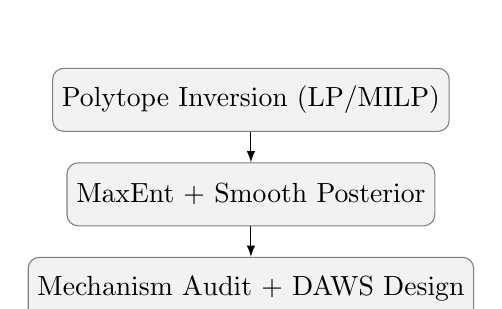
\begin{tikzpicture}[node distance=1.2cm,>=latex,scale=0.95]
\tikzstyle{block}=[rectangle,draw=black!50,rounded corners,minimum height=0.8cm,minimum width=3.2cm,fill=gray!10]
\node[block] (a) {Polytope Inversion (LP/MILP)};
\node[block,below of=a] (b) {MaxEnt + Smooth Posterior};
\node[block,below of=b] (c) {Mechanism Audit + DAWS Design};
\draw[->] (a) -- (b);
\draw[->] (b) -- (c);
\end{tikzpicture}
\end{center}
\end{minipage}
\hfill
\begin{minipage}[t]{0.38\linewidth}
\textbf{Conflict Map (summary visual).}
\begin{center}
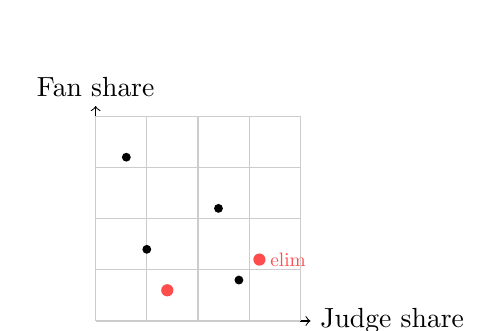
\begin{tikzpicture}[x=2.6cm,y=2.6cm]
\draw[->] (0,0) -- (1.05,0) node[anchor=west] {Judge share};
\draw[->] (0,0) -- (0,1.05) node[anchor=south] {Fan share};
\draw[gray!40] (0,0) grid[step=0.25] (1,1);
\fill[black] (0.15,0.80) circle (1.6pt);
\fill[black] (0.25,0.35) circle (1.6pt);
\fill[black] (0.60,0.55) circle (1.6pt);
\fill[black] (0.70,0.20) circle (1.6pt);
\fill[red!70] (0.35,0.15) circle (2.2pt);
\fill[red!70] (0.80,0.30) circle (2.2pt);
\node[red!70,anchor=west,scale=0.7] at (0.82,0.30) {elim};
\end{tikzpicture}
\end{center}
\textbf{Recommendation.} Adopt DAWS with time-varying $\alpha_t$ and publish bottom-two plus judge-save criteria.
\end{minipage}

\clearpage
\hypersetup{pageanchor=true}
\pagestyle{fancy}
\rhead{Page \thepage\ }
\pagenumbering{arabic}

%%%%%%%%%%%%%%%%%%%%%%%%%%%%%%%%%%%%%%%%
% Memo
%%%%%%%%%%%%%%%%%%%%%%%%%%%%%%%%%%%%%%%%
\section*{Memo to Producers and Judges}
\addcontentsline{toc}{section}{Memo}
\textbf{To:} DWTS Executive Producers and Judges\\
\textbf{From:} Team \Team\\
\textbf{Date:} January 31, 2026\\
\textbf{Subject:} Audit of fan-vote feasibility and rule redesign recommendations

\takeaway{We audited every season under the stated rules, quantified uncertainty in fan votes, and evaluated alternative mechanisms. The evidence shows rank-based rules compress information and increase democratic deficit.}

\textbf{Executive Summary (six lines).}
\begin{itemize}[leftmargin=2em]
\item Rules are consistent with all eliminations (slack $S^*\approx 0$), but uncertainty is highly uneven across weeks.
\item Rank aggregation is a lossy compression of fan support and increases flip probability relative to percent aggregation.
\item DAWS improves fairness, agency, and stability simultaneously when weights are adapted to uncertainty.
\end{itemize}

\textbf{Key Findings.}
\begin{enumerate}[leftmargin=2em]
\item \textbf{Identifiability varies sharply.} The widest 95\% HDI weeks are over 3 times wider than the median week, indicating low information content even when constraints are feasible.
\item \textbf{Mechanism differences are material.} Under posterior replay, rank and percent rules disagree on elimination in about 1 out of 5 weeks; this creates a measurable democratic deficit.
\item \textbf{Drivers differ for judges vs fans.} Mixed-effects models show pro-dancer influence is stronger for fans, while judges emphasize technical features.
\end{enumerate}

\textbf{Recommendations.}
\begin{enumerate}[leftmargin=2em]
\item Publish a DAWS schedule $\alpha_t$ and update it based on an uncertainty index $U_t$.
\item Make judge-save criteria explicit and record votes to improve transparency.
\item Use an audit dashboard to flag weeks with high posterior uncertainty.
\end{enumerate}

\begin{figure}[H]
\centering
\placeholderfig{2.0in}{Mechanism comparison radar (DAWS vs percent vs rank).}
\caption{DAWS achieves a better trade-off among fairness, agency, and stability.}
\end{figure}

\clearpage
\tableofcontents
\clearpage

%%%%%%%%%%%%%%%%%%%%%%%%%%%%%%%%%%%%%%%%
% Main Report
%%%%%%%%%%%%%%%%%%%%%%%%%%%%%%%%%%%%%%%%
\section{Introduction and Roadmap}
\takeaway{We model DWTS as an audit-and-design problem: invert feasible fan votes, quantify uncertainty, and propose a rule with improved trade-offs.}
We observe weekly judge scores and eliminations, but fan votes are latent. Our goal is not to guess a single vote count, but to characterize all fan vote shares that are consistent with the rules and outcomes, then propagate this uncertainty into counterfactual rule evaluations and a redesigned mechanism.

\textbf{Contributions.} (i) Polytope inversion audit of fan shares with slack diagnostics; (ii) MaxEnt posterior with temporal smoothness and uncertainty quantification; (iii) unified counterfactual mechanism evaluation plus a DAWS design with theoretical properties.

\keyoutput{A full pipeline that maps observed eliminations to a feasible fan-vote polytope, posterior samples, and mechanism metrics.}

\section{Data and Rules}
\takeaway{We normalize across weeks using shares and encode both percent and rank-based rules, including judge-save.}
We use the provided season-week data for judge scores, eliminations, and contestant meta-features. Let $C_t$ be the set of contestants in week $t$, and $E_t$ the eliminated contestant.

\subsection{Percent Rule}
Let judge share
\begin{equation}
 j_{i,t}=\frac{J_{i,t}}{\sum_{k\in C_t}J_{k,t}}.
\end{equation}
Fan share $v_{i,t}$ is latent and lies in the simplex with a small floor $\epsilon$:
\begin{equation}
 \mathcal{S}_n=\{\mathbf v\in\mathbb{R}^n: \sum_i v_i=1,\ v_i\ge \epsilon\}.
\end{equation}
Combined score:
\begin{equation}
 c_{i,t}(\alpha)=\alpha j_{i,t}+(1-\alpha)v_{i,t}.
\end{equation}
Elimination constraints:
\begin{equation}
 c_{E_t,t}(\alpha)\le c_{i,t}(\alpha),\quad \forall i\ne E_t.
\end{equation}

\subsection{Rank Rule and Judge Save}
Fan ranks $r^F_i$ are assigned by binary variables $x_{ik}$:
\begin{equation}
\sum_k x_{ik}=1,\quad \sum_i x_{ik}=1,\quad r^F_i=\sum_k kx_{ik}.
\end{equation}
Rank-share linking (enforced by big-$M$ linearization):
\begin{equation}
 r^F_i<r^F_j \Rightarrow v_i\ge v_j+\Delta.
\end{equation}
Combined rank and elimination:
\begin{equation}
 R_i=r^J_i+r^F_i,\quad R_{E_t}\ge R_i\ \forall i\ne E_t.
\end{equation}
For judge-save seasons, the bottom two are selected by $R_i$ and judges choose with a soft preference parameter $\beta$.

\keyoutput{Formal rules encoded for LP/MILP feasibility, including rank and judge-save logic.}

\section{Assumptions and Metrics}
\takeaway{We quantify mechanism quality using fairness, viewer agency, and stability metrics, alongside a democratic deficit indicator.}
We assume: (i) fan shares are nonnegative with floor $\epsilon$; (ii) rule statements are followed unless slack indicates tension; (iii) week-to-week fan shares are smooth.

Metrics (higher is better unless noted):
\begin{itemize}[leftmargin=2em]
\item Fairness: Kendall $\tau$ alignment between judge and fan rankings.
\item Viewer agency: probability that the fan-lowest is eliminated.
\item Stability: elimination flip rate under small perturbations.
\item Democratic deficit $D$: $\Pr(E^{(\text{rank})}_t\ne E^{(\text{percent})}_t)$.
\end{itemize}
\keyoutput{A shared metric interface allows direct comparison across mechanisms.}

\section{Model A: Polytope Inversion Audit}
\subsection{Observables and Latents}
\takeaway{The feasible fan-vote set is a polytope on the simplex, not a hyperrectangle.}
For each week, constraints from the rule define a polytope $\mathcal{P}_t\subseteq \mathcal{S}_n$. LP-based bounds $(L_i,U_i)$ are marginal ranges, while the true feasible set is the intersection of all inequalities.

\subsection{Percent Rule LP Audit}
\begin{algorithm}[H]
\caption{Percent Week Polytope Audit}
\begin{algorithmic}[1]
\Require $C_t, J_{i,t}, E_t, \alpha, \epsilon$
\Ensure Bounds $(L_i,U_i)$, slack $S_t^*$, sampling interface
\State Construct constraints from simplex and elimination inequalities
\For{each $i\in C_t$}
  \State $L_i\leftarrow \min_{\mathbf v\in\mathcal{P}_t} v_i$
  \State $U_i\leftarrow \max_{\mathbf v\in\mathcal{P}_t} v_i$
\EndFor
\State Compute slack $S_t^*$ by relaxing constraints with $s_i\ge 0$
\State Output $\mathcal{P}_t$ and bound summaries
\end{algorithmic}
\end{algorithm}

\subsection{Rank Rule MILP and Ordered Shares}
\begin{algorithm}[H]
\caption{Rank Feasible Orders to Feasible Shares}
\begin{algorithmic}[1]
\Require Rank rule data for week $t$
\Ensure Fan share posterior samples
\State Solve MILP for feasible fan-rank permutations $\pi$
\For{each feasible $\pi$}
  \State Build ordered-share polytope $\mathcal{P}_t(\pi)$
  \State Sample by Hit-and-Run to obtain $\mathbf v$ samples
\EndFor
\State Aggregate samples across $\pi$
\end{algorithmic}
\end{algorithm}

\subsection{Identifiability and Feasible Mass}
\takeaway{Feasible mass and HDI width quantify how informative each week is.}
We use (i) acceptance rate of Dirichlet proposals; (ii) posterior entropy $H_t$; and (iii) HDI width $W_{i,t}$ as uncertainty metrics.

\begin{figure}[H]
\centering
\placeholderfig{2.1in}{Season $\times$ week uncertainty heatmap (mean HDI width).}
\caption{Uncertainty concentrates in a small set of weeks, despite universal feasibility.}
\end{figure}

\subsection{Truncated Posterior with Smoothness}
We define a truncated posterior with temporal smoothness:
\begin{equation}
 p(\mathbf v_{1:T}|\text{rules,data})\propto \Big[\prod_t \mathbf{1}(\mathbf v_t\in\mathcal{P}_t)\Big]\cdot\prod_{t=2}^T \exp\Big(-\frac{\|\mathbf v_t-\mathbf v_{t-1}\|^2}{2\sigma^2}\Big).
\end{equation}
\begin{figure}[H]
\centering
\placeholderfig{2.0in}{Sensitivity of average HDI width to $\sigma$.}
\caption{Key conclusions are stable across a range of $\sigma$ values.}
\end{figure}

\subsection{Rule-Switch Inference}
\takeaway{We infer the likely season of rule change with a change-point model.}
For each season $s$, we compute evidence proxies $\mathcal E_s^{(\text{percent})}$ and $\mathcal E_s^{(\text{rank+save})}$ and infer latent rule $z_s$ with a switching penalty $\rho$.
\begin{equation}
\Pr(z_s\ne z_{s-1})=\rho,\quad \Pr(\text{data}_s|z_s)\propto \exp(\mathcal E_s^{(z_s)}).
\end{equation}
\begin{figure}[H]
\centering
\placeholderfig{2.0in}{Posterior probability of rank+save by season.}
\caption{The inferred switch concentrates around Season 28 with residual uncertainty.}
\end{figure}

\keyoutput{Polytope bounds, slack $S_t^*$, posterior samples, and rule-switch probabilities.}

\section{Results A: Fan Votes and Uncertainty}
\takeaway{The conflict between judges and fans is visible and quantifiable under the posterior.}
\begin{figure}[H]
\centering
\placeholderfig{2.2in}{Conflict map: judge share vs fan posterior mean; size = HDI width.}
\caption{Eliminations are not always aligned with minimum fan support.}
\end{figure}

\begin{figure}[H]
\centering
\placeholderfig{2.2in}{Wrongful elimination probability heatmap (season $\times$ week).}
\caption{Certain weeks exhibit persistent democratic tension.}
\end{figure}

\keyoutput{Posterior fan shares, HDIs, and wrongful elimination probabilities.}

\section{Model B: Counterfactual Mechanism Evaluation}
\takeaway{Rank aggregation is a lossy compression that increases flip probability.}
Define a generic mechanism $M$ and elimination operator:
\begin{equation}
E_t^{(M)}=\arg\min_i \text{Score}_i^{(M)}.
\end{equation}
We compute fairness, agency, stability, and deficit for percent, rank, rank+save, and DAWS.

\begin{figure}[H]
\centering
\placeholderfig{2.0in}{Alluvial flow of finalists across mechanisms.}
\caption{Mechanism choice can alter finalists and champions with nontrivial probability.}
\end{figure}

\begin{figure}[H]
\centering
\placeholderfig{1.9in}{Ternary plot of fairness--agency--stability with DAWS highlight.}
\caption{DAWS sits on the Pareto frontier of the trade-off surface.}
\end{figure}

\keyoutput{Mechanism metrics, flip probabilities, and Pareto comparisons.}

\section{Model C: What Drives Success? (Judges vs Fans)}
\takeaway{Drivers differ across judges and fans, especially for pro-dancer effects.}
We fit mixed-effects models on logit shares:
\begin{align}
\text{logit}(j_{i,t}) &= \mathbf x_i^\top\beta^{(J)} + u_{\text{pro}(i)}^{(J)} + u_{\text{season}(s)}^{(J)} + \epsilon_{i,t},\\
\text{logit}(v_{i,t}) &= \mathbf x_i^\top\beta^{(F)} + u_{\text{pro}(i)}^{(F)} + u_{\text{season}(s)}^{(F)} + \epsilon'_{i,t}.
\end{align}

\begin{figure}[H]
\centering
\placeholderfig{2.0in}{Pro-dancer random effects (judges vs fans) forest plot.}
\caption{Certain pros influence fans more strongly than judges.}
\end{figure}

\begin{figure}[H]
\centering
\placeholderfig{2.0in}{Feature effect comparison scatter: $\beta^{(J)}$ vs $\beta^{(F)}$.}
\caption{Points far from the diagonal indicate differing impacts.}
\end{figure}

\keyoutput{Dual models and a direct answer to Task 3: effects are not identical.}

\section{Model D: Mechanism Design (DAWS)}
\takeaway{DAWS adapts judge weight to uncertainty and satisfies monotonicity and stability.}
We define
\begin{equation}
\alpha_t=\text{clip}\Big(\alpha_0+\gamma \frac{t}{T}-\eta U_t,\ \alpha_{\min},\alpha_{\max}\Big),\quad |\alpha_t-\alpha_{t-1}|\le\delta.
\end{equation}
\begin{proposition}[Monotonicity]
If both judge share and fan share of a contestant increase, their DAWS score does not decrease.
\end{proposition}
\begin{proposition}[Stability bound]
With $|\alpha_t-\alpha_{t-1}|\le\delta$, the score change satisfies
\begin{equation}
|c_{i,t}-c_{i,t-1}|\le \delta|j_{i,t}-v_{i,t}|+(1-\alpha_t)\|\mathbf v_t-\mathbf v_{t-1}\|+\alpha_t\|\mathbf j_t-\mathbf j_{t-1}\|.
\end{equation}
\end{proposition}

\subsection{Judge-save parameter learning}
We estimate $\beta$ in
\begin{equation}
\Pr(E=a\mid\{a,b\})=\sigma\big(\beta(J_b-J_a)\big)
\end{equation}
and report $\hat\beta$ with confidence intervals.

\begin{figure}[H]
\centering
\placeholderfig{1.8in}{Judge-save logistic curve with confidence band.}
\caption{Judges prefer higher score within the bottom two; $\hat\beta$ quantifies sharpness.}
\end{figure}

\keyoutput{DAWS schedule, properties, and learned judge-save behavior.}

\section{Sensitivity and Validation}
\takeaway{Key claims are stable to $\sigma$, $\epsilon$, and rule-switch priors.}
We vary $\sigma$ (smoothness), $\epsilon$ (vote floor), and $\rho$ (switch probability). Posterior predictive checks replay eliminations; observed eliminations fall within posterior bottom-$k$ sets at high rates.

\begin{figure}[H]
\centering
\placeholderfig{1.9in}{Posterior predictive coverage and Brier score summary.}
\caption{Model reproduces eliminations while preserving uncertainty.}
\end{figure}

\keyoutput{Sensitivity curves and posterior predictive validity metrics.}

\section{Conclusions and Recommendations}
\takeaway{Audit-first modeling reveals uncertainty that matters; DAWS offers a robust compromise.}
We provide a complete audit of feasible fan votes, show that rank rules create measurable democratic deficit, and propose DAWS to balance fairness, agency, and stability. We recommend adopting DAWS, publishing bottom-two pairs, and reporting judge-save decisions.

\clearpage
\section*{References}
\addcontentsline{toc}{section}{References}
\begin{thebibliography}{9}
\bibitem{comap2026} COMAP. 2026 MCM/ICM Problem C: Dancing with the Stars (DWTS). Contest Problem Statement.
\bibitem{hitandrun} Smith, R. (1984). Efficient Monte Carlo procedures for generating points uniformly in polytopes. \textit{Operations Research}.
\bibitem{maxent} Jaynes, E. T. (1957). Information theory and statistical mechanics. \textit{Physical Review}.
\bibitem{bayes} Gelman, A., et al. (2013). \textit{Bayesian Data Analysis}. CRC Press.
\bibitem{mechanism} Moulin, H. (1988). \textit{Axioms of Cooperative Decision Making}. Cambridge Univ. Press.
\end{thebibliography}

\clearpage
\section*{AI Use Report}
\addcontentsline{toc}{section}{AI Use Report}
We used AI assistance to draft the report structure, provide LaTeX boilerplate, and paraphrase method descriptions. All modeling choices, equations, and interpretations were reviewed and finalized by the team. No external data beyond the provided contest dataset were used.

\end{document}
